\documentclass[12pt, hyperref={unicode}]{beamer}

\usepackage[T1]{fontenc}
\usepackage[utf8]{inputenc}
\usepackage[slovene]{babel}

\usepackage{pgfpages}
\usepackage{bookmark}
\usepackage{graphicx}%za vstavljanje slik
\usepackage{array}%za tabele
\usepackage{enumerate}
\usepackage{lmodern}
\usepackage{amsfonts}
\usepackage{amsmath}


\mode<presentation>

%tema
\usetheme{Berlin}
\usecolortheme{default}
\useinnertheme[shadows]{rounded}
\useoutertheme{infolines}
\setbeamertemplate{navigation symbols}{}
\beamertemplatenavigationsymbolsempty

%pisava
\usepackage{palatino}
\usefonttheme{serif}
%serif doda podaljšane črtice pri I

\newtheorem{definicija}{Definicija}
\newtheorem{izrek}{Izrek}
\newtheorem{trditev}{Trditev}
\newtheorem{posledica}{Posledica}
\newtheorem{lema}{Lema}
\newtheorem{dokaz}{Dokaz}
\newtheorem{domneva}{Domneva}


\title{(Osnovne) Igre ustvarjanja omrežja}
\subtitle{Dolga predstavitev diplome}
\author{Peter Milivojević}
\institute[FMF]{Fakulteta za matematiko in fiziko}
\date{8. \ april \ 2024}

\begin{document}

% ===================================================================
\begin{frame}
    \titlepage
\end{frame}
% -------------------------------------------------------------------


% -------------------------------------------------------------------
\begin{frame}
   
  \frametitle{(Osnovne) Igre ustvarjanja omrežja}
  Omrežje lahko ustvarimo na več načinov in pri različnih optimizacijskih pogojih.
  Omrežje lahko ustvari centralna avtoriteta in tako doseže socialni optimum ali pa
  več igralcev, kjer vsak poskuša doseči svoj sebični optimum v dani situaciji.
  V diplomski nalogi se bom pretežno ukvarjal z dvema verzijama osnovnih iger ustvarjanja omrežja:
  \vspace{1mm}
  \begin{itemize}
    \item Maksimalna oddaljenost
    \item Vsota oddaljenosti oz. povprečna oddaljenost
  \end{itemize}

\end{frame}
% -------------------------------------------------------------------

% -------------------------------------------------------------------
\begin{frame}
   
    \frametitle{Uporabne definicije}
    \begin{definicija}
    $Graf$ je urejen par $G = (V, E)$, kjer je V neprazna množica točk grafa G in E množica povezav grafa G, pri čemer je vsaka povezava par točk.
    \end{definicija}

    \begin{definicija}
    $Graf$ G je povezan, če za vsak par vozlišč $u, v \in V(G)$ obstaja pot od $u$ do $v$.
    \end{definicija}

\end{frame}
% -------------------------------------------------------------------

% -------------------------------------------------------------------
\begin{frame}
   
    \frametitle{Uporabne definicije}
    \begin{definicija}
    Naj bo $G$ povezan graf in $v \in V(G)$. Stopnja točke $v$ je enaka vsoti števila povezav, ki imajo to točko za krajišče (in dvojnega števila zank v tej točki).
    Označimo jo z $deg(v)$.
    \end{definicija}
    
    \begin{definicija}
    Naj bo $G$ povezan graf in $u, v \in V(G)$. Razdalja $d(u, v)$ je dolžina najkrajše poti med vozliščema $u$ in $v$ (t.j. razdalja med $u$ in $v$) v grafu $G$.
    \end{definicija}

\end{frame}
% -------------------------------------------------------------------

% -------------------------------------------------------------------
\begin{frame}
   
    \frametitle{Uporabne definicije}
    \begin{definicija}
    Naj bo $G$ povezan graf. Premer grafa $G$ je definiran kot $\text{diam}(G) = \max_{u, v \in V(G)} d(u, v)$, kjer je $d(u, v)$ razdalja med vozliščema $u$ in $v$ v grafu $G$.
    \end{definicija}
    
    \begin{definicija}
    Naj bo $G$ povezan graf. Lokalni premer točke $v$ grafa $G$ je definiran kot $\epsilon_G(v) = \max_{u \in V(G)} d(u, v)$, kjer je $d(u, v)$ razdalja med vozliščema $u$ in $v$ v grafu $G$.
    \end{definicija}
    
    

\end{frame}
% -------------------------------------------------------------------

% -------------------------------------------------------------------
\begin{frame}
   
    \frametitle{Uporabne definicije}
    \begin{definicija}
    Povezan graf $G$ ima prerezno vozlišče $v$, če graf $G - v$ ni povezan.
    \end{definicija}

    \begin{definicija}
    Naj bo $G$ povezan graf z n vozlišči. Wienerjev indeks $W = W(G)$ je definiran
    kot vsota vseh razdalj med vozlišči.
    $$W(G) = \sum_{i=1}^{n} \sum_{j=1}^{i} d_{ij} = \frac{1}{2} \sum_{i=1}^{n} \sum_{j=1}^{n} d_{ij}$$
    kjer $d_{ij}$ označuje dolžino najkrajše poti med vozliščem $i$ in $j$.
    \end{definicija}

\end{frame}
% -------------------------------------------------------------------

% -------------------------------------------------------------------
\begin{frame}
   
  \frametitle{Strateška igra}
  \begin{definicija}
    Strateška igra s funkcijo preferenc je trojica $(N, (A_i)_{i\in N} , (u_i)_{i\in N})$ pri čemer:
\begin{itemize}
    \item $N$ je množica igralcev, v našem primeru je to število točk v grafu
    \item Za vsakega igralca $i \in N$ je $A_i$ neprazna množica njegovih akcij, med katerimi v danem trenutku izbera igralec $i$
    \item Za vsakega igralca $i \in N$ je $u_i$ funkcija preferenc na $A_i$. Torej $u_i : A_i \to \mathbb{R}$ v splošnem in $u_i : A_i \to \mathbb{N}$ v našem primeru.
\end{itemize}
\end{definicija}
Za funkcijo preferenc lahko zapišemo sledeče relacije.

$\forall a,b \in A_i:$
\begin{itemize}
    \item $(u(a) \geq u(b) \Rightarrow a)$ je vsaj tako dobro kot $b$
    \item $(u(a) > u(b) \Rightarrow a)$ je boljše kot $b$
    \item $(u(a) = u(b) \Rightarrow b)$ indiferenten med $a$ in $b$
\end{itemize}

\end{frame}
% -------------------------------------------------------------------

% -------------------------------------------------------------------
\begin{frame}
   
    \frametitle{Definiciji ravnovesja}
    \begin{definicija}
    Graf je v \textit{ravnotežju glede na vsoto razdalj}, če za vsako povezavo $vw$ in
    za vsako vozlišče $w'$ zamenjava povezave $vw$ s povezavo $vw'$ ne zmanjša
    celotne vsote razdalj od vozlišča $v$ do vseh ostalih vozlišč.
    \end{definicija}
        
    \begin{definicija}
    Graf je v \textit{ravnotežju glede na maksimalno razdaljo}, če za vsako povezavo $vw$
    in za vsako vozlišče $w'$ zamenjava povezave $vw$ s povezavo $vw'$ ne zmanjša
    lokalnega premera vozlišča $v$. Nadalje odstranitev povezave $vw$ poveča
    lokalni premer vozlišča $v$.
    \end{definicija}

\end{frame}
% -------------------------------------------------------------------

% -------------------------------------------------------------------
\begin{frame}
   
    \frametitle{Definiciji kritičnosti in stabilnosti}  
    \begin{definicija}
    Naj bo $G$ povezan graf. Graf $G$ je \textit{kritičen za odstranitev povezave},
    če odstranitev katere koli povezave $uv \in E(G)$ poveča lokalni premer vozlišča $v$ in vozlišča $u$.
    \end{definicija}
    
    \begin{definicija}
    Naj bo $G$ povezan graf. Graf $G$ je \textit{stabilen za dodajanje povezave},
    če dodajanje katere koli povezave $uv \in E(G)$ ne zmanjša lokalnega premera vozlišča $v$ in vozlišča $u$.
    \end{definicija}

\end{frame}
% -------------------------------------------------------------------

% -------------------------------------------------------------------
\begin{frame}

  \frametitle{Ceni anarhije in stabilnosti}
  Ceni anarhije (PoA) in stabilnosti (PoS) merita, kako se učinkovitost sistema poslabša zaradi sebičnega vedenja njegovih igralcev.
  Cena anarhije je razmerje med vrednostjo/ceno, iz socialnega vidika (skupnega vidika vseh igralcev), najslabšega ravnovesja in socialno ceno optimalnega izida.
  Cena stabilnosti igre pa je razmerje med najboljšo socialno ceno ravnovesja in socialno ceno optimalnega izida.\\
  Socialno ceno grafa bomo definirali kot vsoto cen vseh vozlišč. Za igro vsote bomo tako socialno ceno definirali kot $SC(G) = 2W(G)$,
  za igro lokalnega premera pa kot $SC(G) = \sum_{i=1}^{n}\epsilon_G(i)$.
\end{frame}
% -------------------------------------------------------------------

% -------------------------------------------------------------------
\begin{frame}

  \frametitle{Ceni anarhije in stabilnosti}
  Tako lahko definiramo sledeče:
  \begin{definicija}
    $PoA = \frac{\text{Socialna cena najslabšega ravnovesja}}{\text{Socialna cena optimalne postavitve}} = \frac{\max_{G\in R} SC(G)}{\min_{G\in A} SC(G)}$
  \end{definicija}
  \begin{definicija}
    $PoS = \frac{\text{Socialna cena najboljšega ravnovesja}}{\text{Socialna cena optimalne postavitve}} = \frac{\min_{G\in R} SC(G)}{\min_{G\in A} SC(G)}$
  \end{definicija}
  Kjer $A$ predstavlja množico vseh možnih povezanih grafov z $|V(G)| = n$ vozlišči in manj ali enako kot $|E(G)| = m$ povezavami.
  Množica $R \subseteq A$ pa predstavlja množico vseh ravnovesnih grafov, ki lahko nastanejo iz začetnih grafov z $n$ vozlišči in $m$ povezavami.
\end{frame}
% -------------------------------------------------------------------

% -------------------------------------------------------------------
\begin{frame}

  \frametitle{Drevesa: skupna vsota razdalj}
  \begin{izrek}
    Če je ravnovesni graf za skupno vsoto razdalj v preprosti igri ustvarjanja
    omrežja drevo, potem ima premer največ $2$ in je kot tak zvezda.
  \end{izrek}

  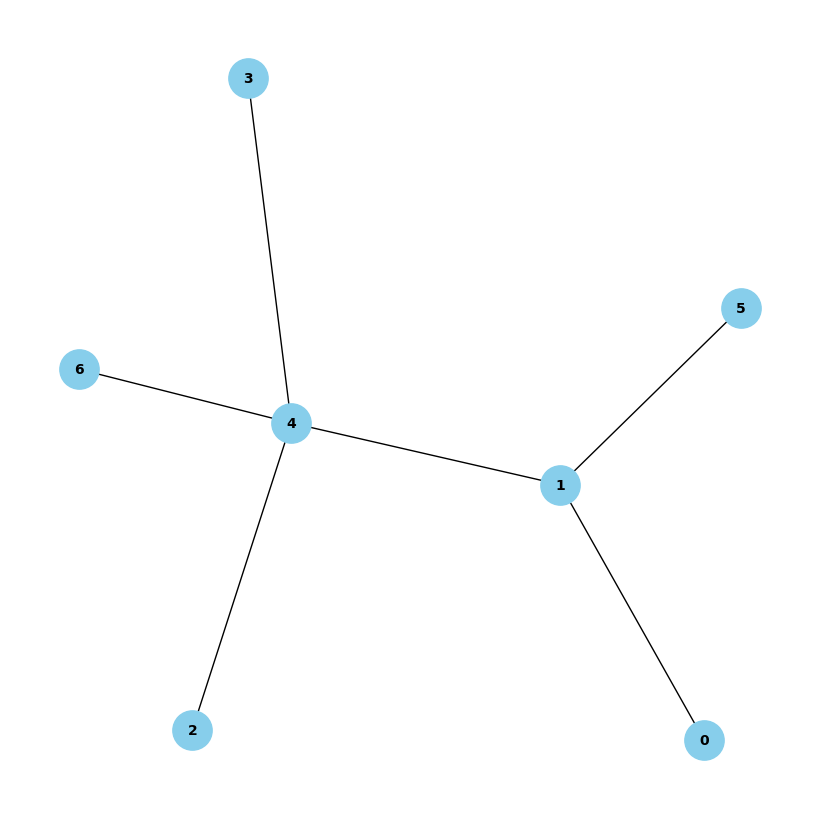
\includegraphics[width=0.3\textwidth]{drevo_1.png}
  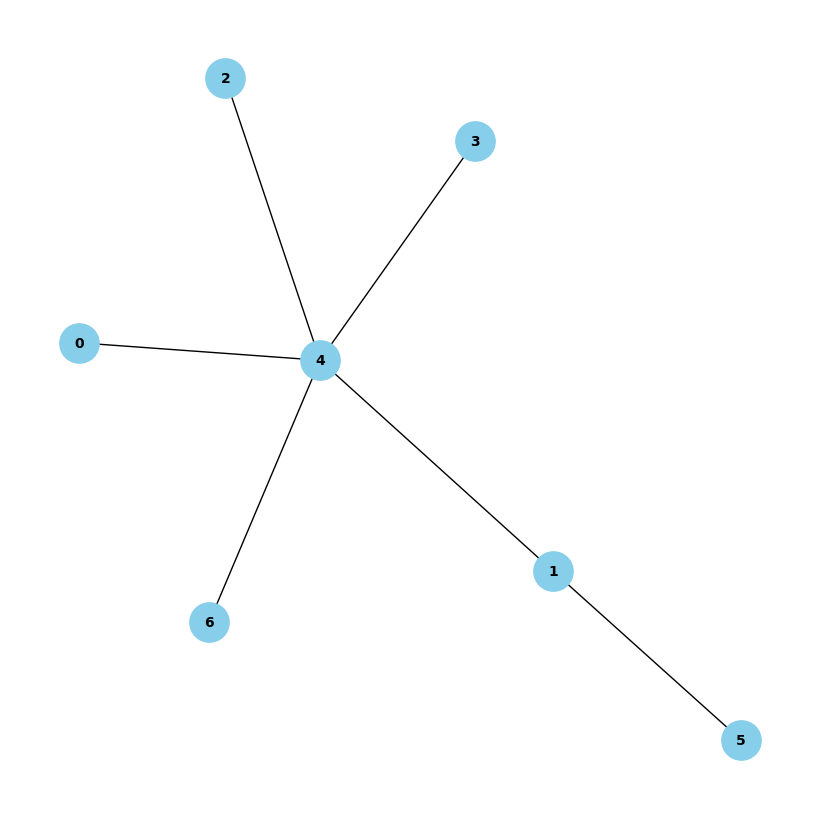
\includegraphics[width=0.3\textwidth]{drevo_2.png}
  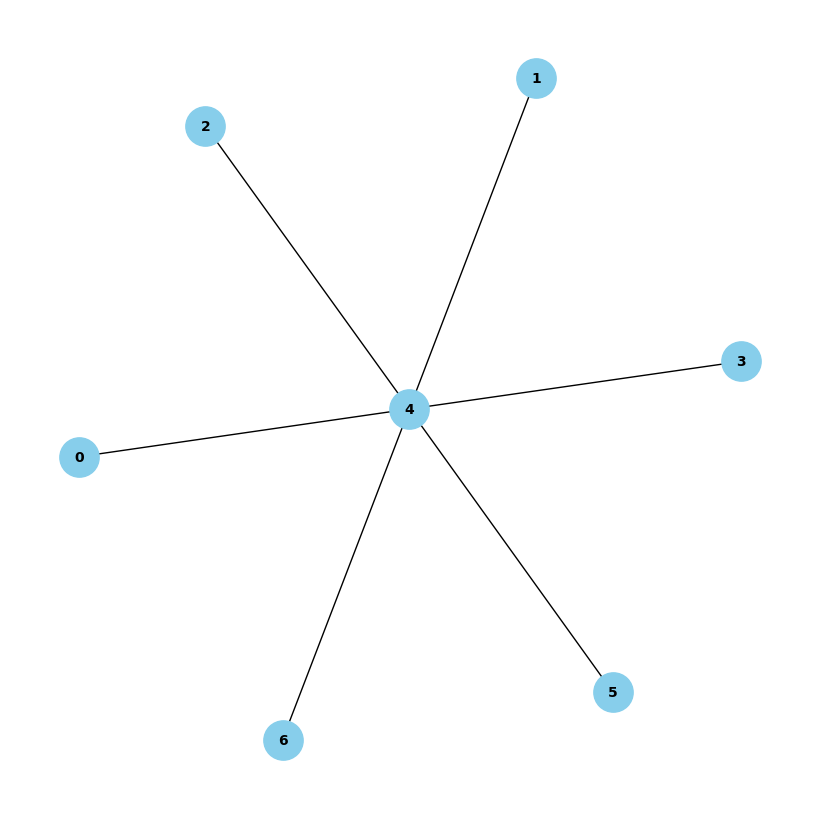
\includegraphics[width=0.3\textwidth]{drevo_3.png}
\end{frame}
% -------------------------------------------------------------------

% -------------------------------------------------------------------
\begin{frame}
   
  \frametitle{Drevesa: maksimalna razdalja}
  \begin{lema}
    V vsakem ravnovesnem grafu igre maksimalne razdalje se lokalni premer za
    katera koli $2$ poljubna vozlišča razlikuje največ za $1$.
  \end{lema}

  \begin{lema}
    Če ima ravnovesni graf za maksimalno razdaljo prerezno vozlišče, potem ima lahko
    samo ena izmed povezanih komponent $G - v$ vozlišče z razdaljo več kot $1$ od $v$.
  \end{lema}

  \begin{izrek}
    Če je ravnovesni graf za maksimalno razdaljo drevo, potem je premer ravnovesnega grafa največ $3$.
  \end{izrek}

\end{frame}
% -------------------------------------------------------------------

% -------------------------------------------------------------------
\begin{frame}
  
  \frametitle{Skupna vsota razdalj: spodnje meje}
  \begin{lema}
    Za vozlišče $v$ z lokalnim premerom $2$, zamenjava sosednje povezave ne izboljša
    vsote razdalj od $v$ do vseh ostalih vozlišč. Prav tako tudi svojega lokalnega premera ne more izboljšati.
  \end{lema}
  \begin{posledica}
    Vsak graf s premerom $2$ ali manj je v \textit{ravnotežju glede na vsoto razdalj}
    in hkrati socialni optimum, zato je cena stabilnosti 1.
  \end{posledica}
  
\end{frame}

% -------------------------------------------------------------------

% -------------------------------------------------------------------
\begin{frame}
  
  \frametitle{Skupna vsota razdalj: spodnje meje}
  \begin{izrek}
    Naj bo $G$ graf z $n$ vozlišči in $m$ povezavami, potem je $W(G) = n^2 - n - m$, če in samo če je premer grafa $2$ ali manj.
  \end{izrek}
  \begin{posledica}
    Za vsak graf $G$ z $n$ vozlišči, $m$ povezavami in premerom večjim od $2$ velja:
    $$W(G) \geq n^2 - n - m + 1.$$
    Enačaj velja kadar ima graf $G$ natanko $2$ vozlišči z lokalnim premerom $3$ in vsa ostala vozlišča z lokalnim premerom $2$.
  \end{posledica}
  
\end{frame}

% -------------------------------------------------------------------

% -------------------------------------------------------------------
\begin{frame}
  
  \frametitle{Skupna vsota razdalj: spodnje meje}
  \begin{columns}
    \column{0.5\textwidth}
    \begin{izrek}
      Obstaja ravnovesni graf za skupno vsoto razdalj s premerom 3.
    \end{izrek}
    \column{0.5\textwidth}
    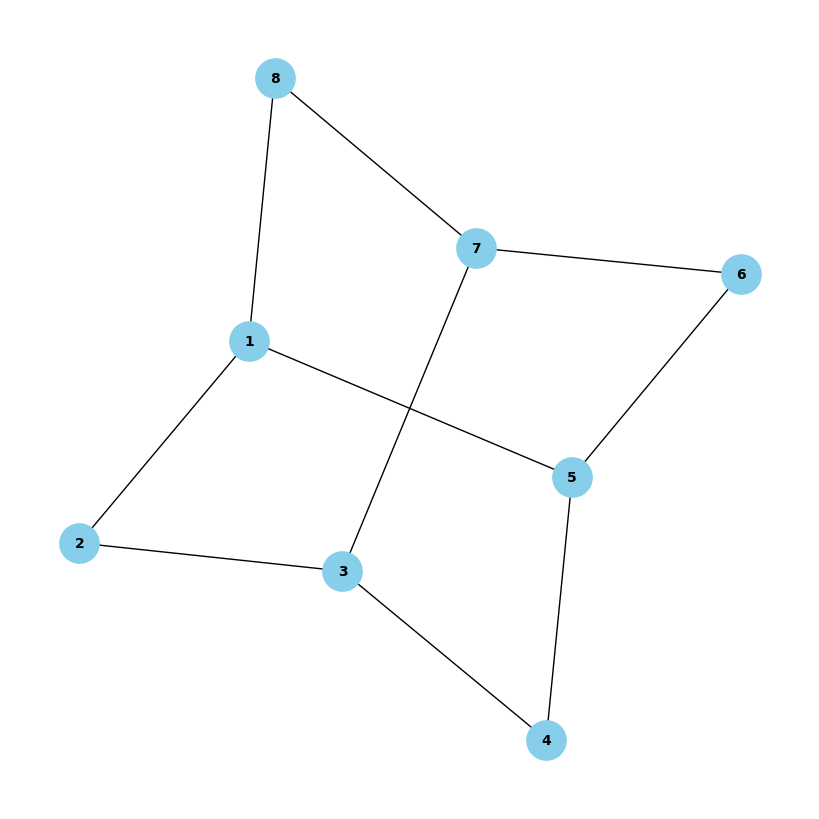
\includegraphics[width=1\textwidth]{vsota_premer_3.png}
  \end{columns}
  
\end{frame}

% -------------------------------------------------------------------

% -------------------------------------------------------------------
\begin{frame}
   
  \frametitle{Skupna vsota razdalj: zgornja meja $2^{O(\sqrt{\log_2 n})}$}
  \begin{izrek}
    Vsak ravnovesni graf za skupno vsoto razdalj ima premer $2^{O(\sqrt{\log_2 n})}$.
  \end{izrek}

  \begin{lema}
    Vsak ravnovesni graf za skupno vsoto razdalj ima premer največ $2 \log_2 n$ ali
    za vsako vozlišče $v$ obstaja povezava $xy$, kjer je $d(u, x) \leq \log_2 n$ in
    zamenjava povezave $xy$ zmanjša vsoto razdalj od $x$ za največ $2n(1 + \log_2 n)$.
  \end{lema}

  \begin{lema}
    V vsakem ravnovesnem grafu za skupno vsoto razdalj dodajanje poljubne povezave
    $uv$ zmanjša vsoto razdalj od $u$ za največ $5n \log n$.
  \end{lema}

\end{frame}
% -------------------------------------------------------------------

% -------------------------------------------------------------------
\begin{frame}

  \frametitle{Maksimalna razdalja}
  \begin{columns}
    \column{0.5\textwidth}
    \begin{izrek}
        Obstaja ravnovesni graf za maksimalno razdaljo s premerom $\Theta(\sqrt{n})$.
    \end{izrek}
    \column{0.5\textwidth}
    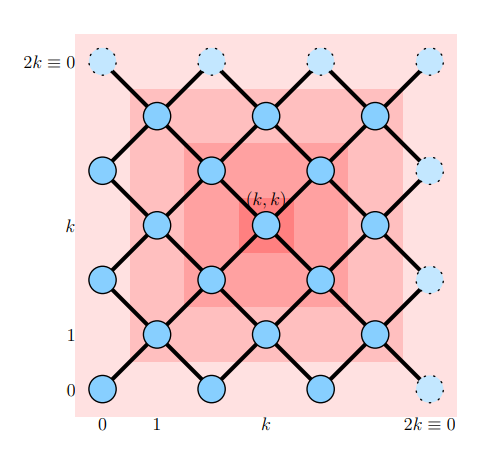
\includegraphics[width=1\textwidth]{Plagiat.png}
  \end{columns}
  
  

\end{frame}
% -------------------------------------------------------------------

% -------------------------------------------------------------------
\begin{frame}

  \frametitle{Povezava z grafi z enotsko razdaljo}
  \begin{izrek}
    Vsak ravnovesni graf $G$ za skupno vsoto razdalj z $n \geq 24$ vozlišč in
    premerom $d > 2 \log_2 n$ inducira podgraf z $\epsilon\text{-skoraj-enotno-razdaljo } G'$
    z $n$ vozlišči in premerom $\Theta\left(\frac{\varepsilon d}{\log_2 n}\right)$ in
    podgraf z $\epsilon\text{-enotno-razdaljo } G'$ z $n$ vozlišči in premerom
    $\Theta\left(\frac{\varepsilon d}{\log_2^2 n}\right)$.
  \end{izrek}

  \begin{domneva}
    Razdaljno skoraj enotni grafi imajo premer $O(\log_2 n)$.
  \end{domneva}


\end{frame}
% -------------------------------------------------------------------





% -------------------------------------------------------------------
\begin{frame}

  \frametitle{Testiranje števila ravnovesji}
  \begin{columns}
    \column{0.5\textwidth}
    \begin{table}
    \scriptsize
    \begin{tabular}{ll}
        Št. ravnovesnih grafov & Št. vozlišč\\
        1                      & 1          \\
        1                      & 2          \\
        2                      & 3          \\
        3                      & 4          \\
        4                      & 5          \\
        7                      & 6          \\
        12                     & 7          \\
        24                     & 8          
    \end{tabular}
    \caption{Maks verzija}
    \end{table}
    \column{0.5\textwidth}
    \begin{table}
    \scriptsize
    \begin{tabular}{ll}
      Št. ravnovesnih grafov & Št. vozlišč\\
      1                      & 1          \\
      1                      & 2          \\
      2                      & 3          \\
      5                      & 4          \\
      15                     & 5          \\
      60                     & 6          \\
      374                    & 7          \\
      4161                   & 8         
    \end{tabular}
    \caption{Verzija vsote}
    \end{table}
\end{columns}


\end{frame}
% -------------------------------------------------------------------

% -------------------------------------------------------------------
\begin{frame}

  \frametitle{Socialni optimum maks verzije}
  \begin{table}
  \tiny
  \begin{tabular}{rrrrrrrrrrrr}
\hline
   n\textbackslash{}e &   n + -1 &   n  &   n + 1 &   n + 2 &   n + 3 &   n + 4 &   n + 5 &   n + 6 &   n + 7 &   n + 8 &   n + 9 \\
\hline
     2 &        2 &         &         &         &         &         &         &         &         &         &         \\
     3 &        5 &       3 &         &         &         &         &         &         &         &         &         \\
     4 &        7 &       7 &       6 &       4 &         &         &         &         &         &         &         \\
     5 &        9 &       9 &       9 &       8 &       8 &       7 &       5 &         &         &         &         \\
     6 &       11 &      11 &      11 &      11 &      10 &      10 &      10 &       9 &       9 &       8 &       6 \\
\hline
\end{tabular}
\caption{Socialni optimum maks verzije}
\end{table}

\end{frame}
% -------------------------------------------------------------------

% -------------------------------------------------------------------
\begin{frame}
  
  \frametitle{Cena anarhije igre vsote}
  \begin{columns}
    \column{0.5\textwidth}
    Pri testiranju grafov do $8$ vozlišč je bila pri večini grafov cena anarhije enaka $1$.
    Izjema so bili grafi z $8$ vozlišči in $10, 11 $ oziroma $12$ povezavami. Cena anarhije je bila
    $\frac{100}{92} = \frac{25}{23}$ za $10$ povezav, $\frac{94}{90} = \frac{47}{45}$ za $11$ povezav
    in $\frac{90}{88} = \frac{45}{44}$  za $12$ povezav.
    \column{0.5\textwidth}
    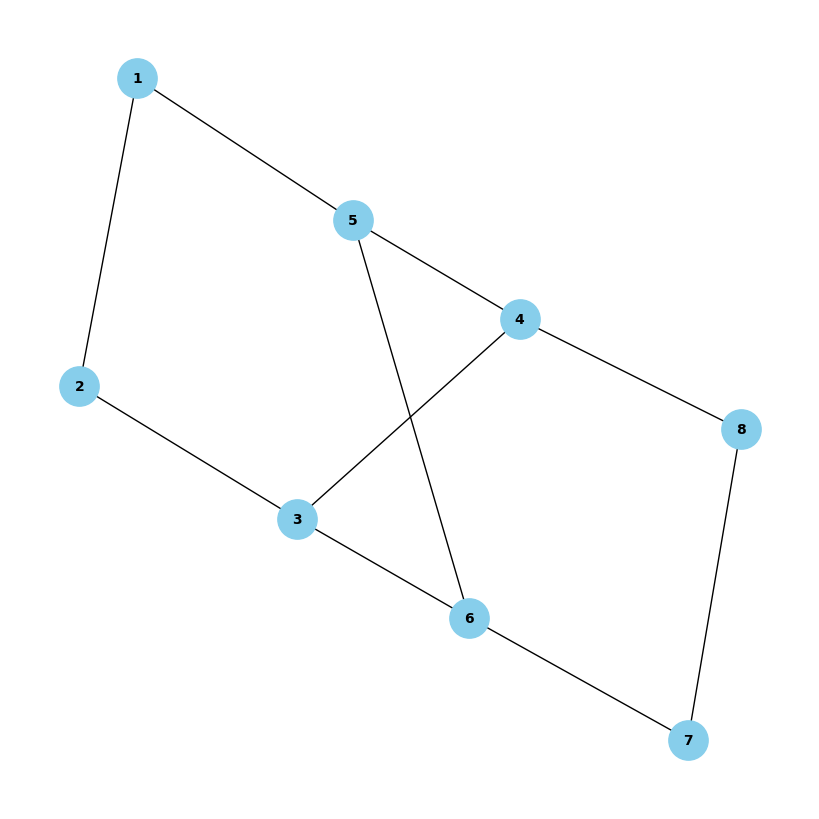
\includegraphics[width=1\textwidth]{8_10_najslabsi.png}
  \end{columns}
  
\end{frame}

% -------------------------------------------------------------------

% -------------------------------------------------------------------
\begin{frame}
  
  \frametitle{Razlike v algoritmih}
  \begin{columns}
    \column{0.5\textwidth}
    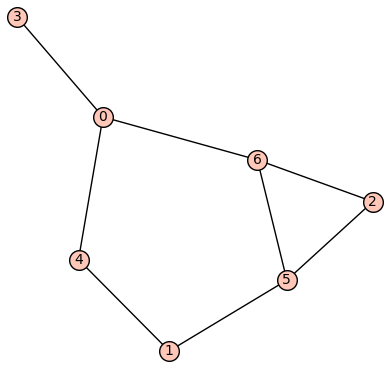
\includegraphics[width=0.8\textwidth]{ciklj_in_d.png}
    \column{0.5\textwidth}
    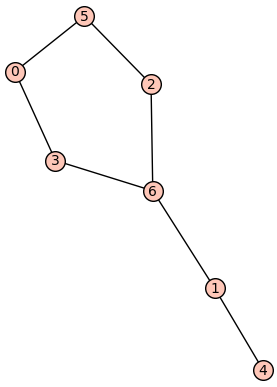
\includegraphics[width=0.8\textwidth]{d_in_cikelj.png}
  \end{columns}
  
\end{frame}

% -------------------------------------------------------------------

% -------------------------------------------------------------------
\begin{frame}
  
  \frametitle{Igra vsote v prostoru}
  \begin{columns}
    \column{0.5\textwidth}
    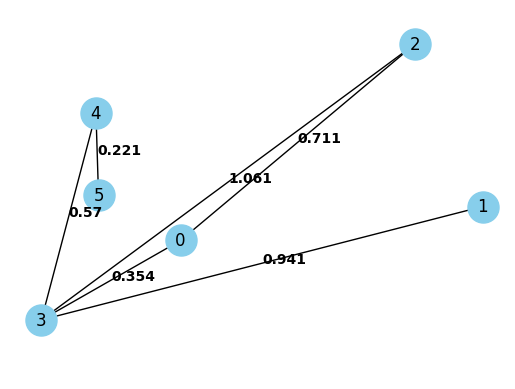
\includegraphics[width=0.8\textwidth]{imput_1.png}
    \column{0.5\textwidth}
    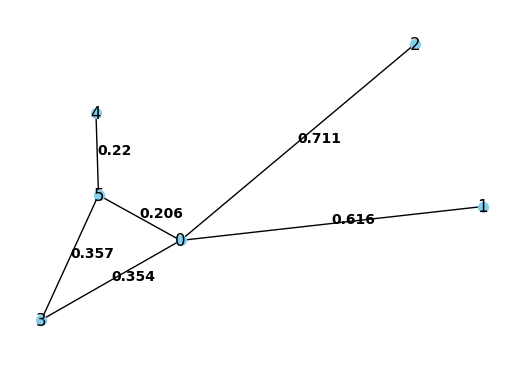
\includegraphics[width=0.8\textwidth]{output_1.png}
    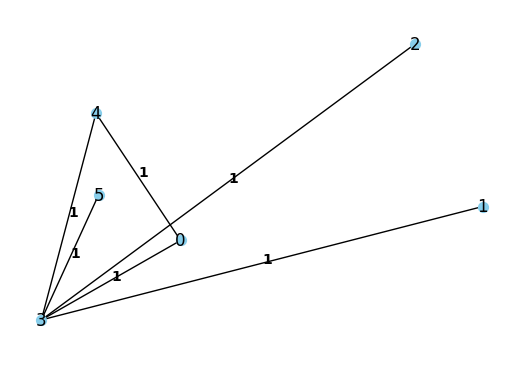
\includegraphics[width=0.8\textwidth]{output_2.png}
  \end{columns}
  
\end{frame}

% -------------------------------------------------------------------

% -------------------------------------------------------------------
\begin{frame}
  
  \frametitle{Igra maksimalne razdalje v prostoru}
  \begin{columns}
    \column{0.5\textwidth}
    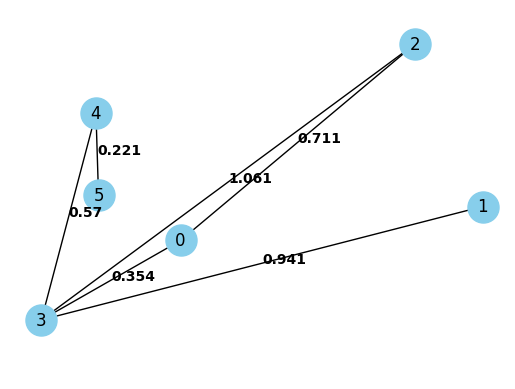
\includegraphics[width=0.8\textwidth]{imput_1.png}
    \column{0.5\textwidth}
    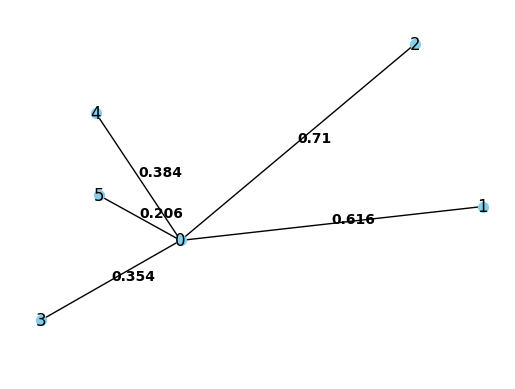
\includegraphics[width=0.8\textwidth]{output_3.png}
    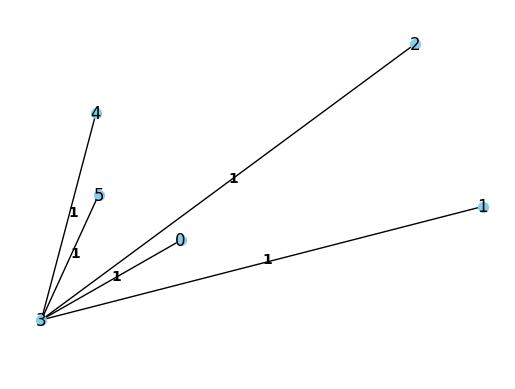
\includegraphics[width=0.8\textwidth]{output_4.png}
  \end{columns}
  
\end{frame}

% -------------------------------------------------------------------



\end{document}